% !TEX root = ../main.tex

\section{Передумови для розгляду диференціальних ігор}
Класична теорія ігор, творцями якої є Джон фон Нейман та Оскар Морґенштерн,
оперує матричними іграми та зв'язаними з ними поняттями. Для них сформульовано та доведено
багато фундаментальних теорем --- наприклад, щодо існування рівноваги Неша. 
Однак, ці результати зовсім не покривають всі можливості формалізувати процеси,
в яких гравці приймають рішення. Наприклад, якщо розглядати задачу про оптимальну траєкторію 
корабля від керованої торпеди, яка його переслідує, то необхідно досліджувати не просто скінченний набір можливих дій
кожного з гравців, а континуум можливих стратегій, кожна з яких відповідає деякій комбінації траєкторій руху корабля та торпеди.

Визначення поняття диференціальної гри буде базуватися на тому, що до їх розв'язання (чи хоча б дослідження)
буде застосовуватися апарат математичного аналізу, як-от теорія диференціальних рівнянь.
Сам термін <<диференціальна гра>> було введено Руфусом Айзексом --- одним з основоположників теорії диференціальних ігор.

Прикладами диференціальних ігор, окрім наведеного вище, є й звичайні спортивні ігри на кшталт футболу,
де, очевидно, недоречно розглядати лише дискретні моменти часу або скінченний набір стратегій,
бо найменше відхилення від таких стратегій (яке, звичайно, може статися через людський фактор),
породжує вже іншу стратегію. Зауважимо, що коли рішення протягом усієї гри приймає лише один гравець,
то така задача фактично стосується \emph{теорії керування} та \emph{варіаційного числення}, тому такі випадки в
теорії ігор не розглядаються. 

\section{Опис ходу гри}
Рішення, що їх приймають гравці, полягають у виборі так званих \emph{керувань}, від яких залежать
\emph{фазові координати}: їх значення у будь-який момент часу повністю визначає хід гри, характеризуючи
положення гравців у деякому просторі --- \emph{фазовому просторі}.
Для визначення результату гри необхідно знати значення фазових координат у початковий момент. Також, в кожен момент часу
гравець має звертати увагу на значення фазових змінних (що, по суті, і означає деяких рух гравців).
В процесі гри фазові координати змінюються. Оскільки розглядається випадок скінченної кількості фазових змінних,
то фазовий простір зручно ототожнювати з координатами точок в $\R^n$ (або в деякій підмножині цього простору).
Поточні значення фазових координат завжди відомі гравцям --- тобто, це ігри з повною інформацією.
Невідомим зазвичай є характер їх зміни: тобто, \emph{керування} фазовими змінними гравцями.
Хід гри характеризується рухом точки у фазовому просторі, причому гра завершується, якщо виконуються деякі умови: наприклад,
потрапляння точки в деяку підмножину простору.

\section{Приклади задання фазових змінних}
Розглянемо приклади задання фазових змінних у випадку керування лише одним об'єктом.
\begin{example}
    Положення матеріальної точки на площині описується двома координатами $x_1$ та $x_2$. 
    Нехай швидкість руху точки є сталою $v$, а гравець обирає напрямок швидкості $\vf$ та може змінювати його у будь-який момент часу --- тобто, $\vf$
    є керуванням. Тоді рух точки описується системою диференціальних рівнянь
    \begin{gather*}
        \begin{cases}
            \d{x_1} = v \cos \vf \\
            \d{x_2} = v \sin \vf
        \end{cases}
    \end{gather*}
    Інший гравець у будь-який момент часу може виміряти значення фазових координат $x_1$ та $x_2$, але закону їх зміни (керування першого гравця) він не знає.
\end{example}
\begin{example}(\cite{1})
    Геометричне положення автомобіля на декартовій площині описується трьома фазовими координатами:
    $x_1, x_2$ --- положення деякої точки автомобіля, $x_3$ --- кут, який утворює вісь вздовж автомобіля
    з деяким фіксованим напрямком --- наприклад, $x_1$.
    \begin{center}
        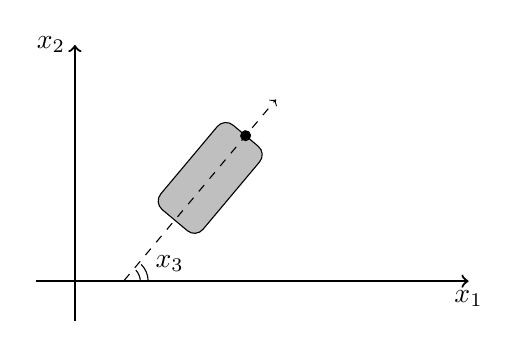
\begin{tikzpicture}
            \draw [->, thick] (-0.5, 0) -- (5, 0);
            \draw [->, thick] (0, -0.5) -- (0, 3);
            \node [below] at (5, 0) {$x_1$};
            \node [left] at (0, 3) {$x_2$};
            \filldraw [fill=lightgray, rounded corners, rotate around={-40:(1,1)}] (1, 1) rectangle (1.7, 2.4);
            \fill [rotate around={-40:(1,1)}] (1.35, 2.4) circle [radius=2pt];
            \draw [->, dashed, rotate around={-40:(1,1)}] (1.35, 0) -- (1.35, 3);
            \draw (0.83, 0) arc (0:44:0.2);
            \draw (0.93, 0) arc (0:45:0.3);
            \node [right] at (0.9, 0.22) {$x_3$};
        \end{tikzpicture}
    \end{center}
    Якщо цей автомобіль є складовою диференціальної гри, то про нього треба знати більше. Нехай гравець керує ним за допомогою педалі акселератора, що
    задає прискорення, та керма, що задає напрямок руху. Нехай $A$ --- максимальне можливе прискорення автомобіля, тоді прискорення може набувати значень
    $A \vf_1$, де $\vf_1 \in [0; 1]$ і знаходиться під контролем гравця-водія. Можна ввести ще одну фазову координату $x_4$ --- швидкість автомобіля.
    Інший гравець у будь-який момент часу знає (чи може виміряти) значення фазових координат, але не значення керування $\vf_1$. Положення керма визначає кривину траєкторії
    руху автомобіля, значення якої, очевидно, є обмеженими. Таким чином, можна ввести кривину як ще одну фазову координату $x_5$
    (фізично --- це кут повороту передніх коліс), керуванням якої є $W \vf_2$, де $\vf_2 \in [-1; 1]$, а $W$ --- максимальна швидкість зміни $x_5$.
    
    Отже, маємо систему, що задає рух автомобіля у деякій диференціальній грі:
    \begin{gather*}
        \begin{cases}
            \d{x_1} = x_4 \cos{x_3} \\
            \d{x_2} = x_4 \sin{x_3} \\
            \d{x_3} = x_4 x_5 \\
            \d{x_4} = A \vf_1, \; \vf_1 \in [0; 1] \\
            \d{x_5} = W \vf_2, \; \vf_2 \in [-1; 1]
        \end{cases}
    \end{gather*}
    Два перших рівняння --- координатний запис швидкості руху автомобіля, третє означає, що швидкість зміни напрямку руху дорівнює добутку швидкості руху на кривину траєкторії,
    а два останні задають керування гравцем швидкості руху та швидкості зміни кривини траєкторії руху. Звісно, вони не є точними з фізичної точки зору (тому що, наприклад, не враховують тертя), але
    є досить простими для аналізу.
\end{example}